
\usepackage{graphicx}
\usepackage{float}

\title{Laboratorium 5 - Sprawozdanie}
\author{Wojciech Makuch}


\maketitle
\section{Zadanie}
Program framework benchmarkujacy dla zaimplementowanego abstrakcyjnego typu danych: tablica haszujaca.
\section{Realizacja}
Program wykonano na bazie zwyklej tablicy alokowanej dynamicznie o zadanym maksymalnym rozmiarze. Rozmiar nie może byc zmienny, ponieważ metody haszujace bazują na operacji dzielenia modulo przez ten rozmiar, jego zmiana spowodowałaby znaczne pogorszenie złożoności obliczeniowej. Program zwiera 2 struktury: pierwsza przechowuje dane(element, wartość), druga to tablica przechowujaca te dane. Program zawiera 2 metody haszujace. Pierwsza z nich bazuje na operacji dzielenia modulo przez maksymalny rozmiar wartosci liczbowej kodu ASCII klucza. Druga metoda wykorzystuje wzor q-(dodany wartosci klucza)/q, gdzie q jest polowa maksymalnego rozmiaru i q jest liczba nieparzysta. Zasada wypelniania tablicy jest nastepujaca:
\begin{enumerate}
	\item WezKlucz
	\item i$\leftarrow$ PierwszeHaszowanie
	\item jeśli tab[i]=0, to wypełnij komórke. \\
	w przypadku przeciwnym:
	\item $j\leftarrow$ DrugieHaszowanie
	\item jeśli tab[i+j]=0, to wypełnij komórkę. \\
	w przypadku przeciwnym:
	\item Wypelnij najblizsza wolno komorkę.
\end{enumerate}
Ponadto program zawiera przeciązenie operatora [] pozwalającego odnieść się do wybranej komórki tablicy haszującej(asocjacyjnej) za pomocą klucza. Algorytm działa na tym samym schemacie, co wypłenianie.
\section{Działanie}
Program tak samo jak poprzednie nie udostępnia użytkownikowi interfesju. Po uruchomieniu jedynie wyswietla dane, które są jednocześnie zapisywane do pliku o nazwie \textsl{pomiar\_czas\_5.txt}. Główna funkcja programu wywołuje jednynie funkcje \textsl{benchmarkuj()}, która zawiera pętle zliczania i zpaisywania uzyskanych wyników.

\section{Wyniki}
Przetestowano czas wypełniania tablicy haszującej elementami losowymi. Uzyskane dane przedstawiono na rys 1. Wynika z nich wprost, że złożoność obliczeniowa wynosi $O(n^{2})$, lecz po aproksymacji widać, ze współczynik przy $x^{2}$ jest bardzo mały(0.0046), co oznacza, że wykres mozna również przyblizyć prostą. Wtedy złożoność obliczeniowa wyniesie $O(n)$. jest to najgorszy możliwy przypadek szukania pustej komórki przechodząc się kolejno po elementach tablicy, co dzieje się dosyć często przy wypełnianiu tablicy tak duzą ilocią elementów. Na rys 2. pokazano ten sam wykres dla mneijszej ilosci danych, Widać tu, że żadna funkcja nie jest ani rosnąca, ani malejąca. Może to sugerować złożoność obliczeniową O(1) dla małej ilości elementów.
\begin{figure}[b!]
\centering
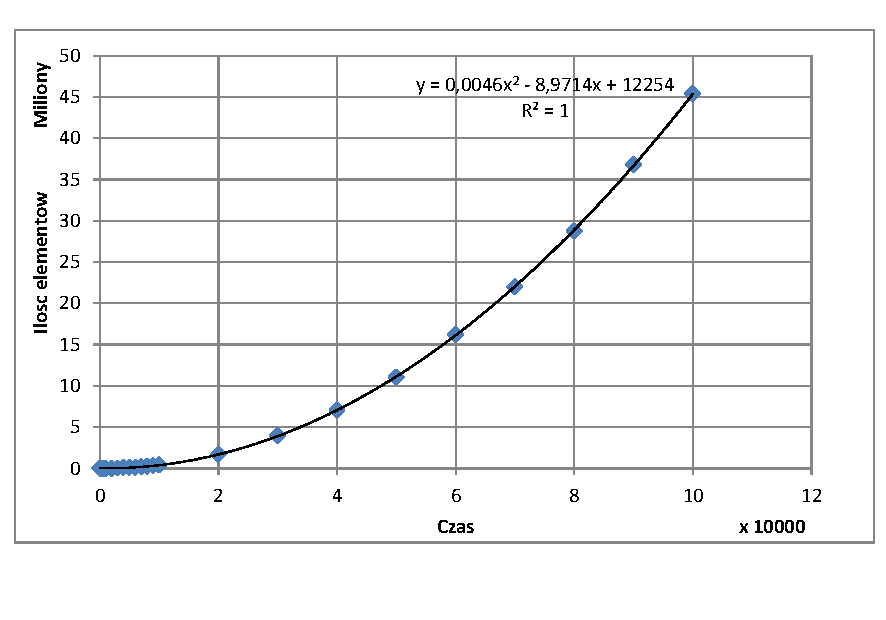
\includegraphics[scale=0.75]{Wykres1.pdf}
\caption{Wykres złożoności obliczeniowej dla dużej ilości elementów.}
\label{fig:wykres1}
\end{figure}
\begin{figure}[t!]
	\centering
	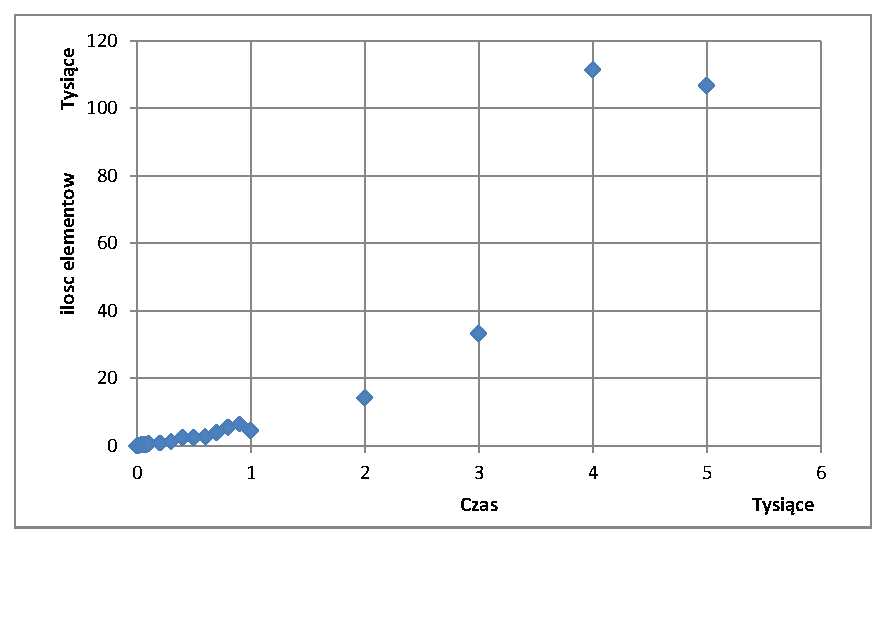
\includegraphics[scale=0.75]{Wykres2.pdf}
	\caption{Wykres złożoności obliczeniowej dla małej ilości elementów}
	\label{fig:wykres2}
\end{figure}
\section{Podsumowanie}
Złozoność obliczeniowa algorytmu wypełniania tablicy haszującej w najgorszym przypadku dla dużej ilości elementów jest $O(n)$ lub $O(n^{2})$ natomiast w najlepszym przypadku dla małej ilości jest $O(1)$.
\section{Komentarz}
Do utworzenia dokumentacji wykorzystano system Doxygen.
Funkcja pomiaru czasu dla systemu Windows pobrana ze strony dr. J. Mierzwy. Program skompilowano w środowisku Code::Blocks. Do stworzonia wykresu posłużono się pakietem MS Excel, sprawozdanie napisano używając systemu \LaTeX.

\end{document}